% -*- root: ../main.tex -*-
\chapter{Consenso e State Machine Replication}
Il principale vantaggio fornito dai sistemi distribuiti rispetto ai sistemi centralizzati sta nel fatto di poter garantire un servizio continuo malgrado \textit{failures} e \textit{malfunzionamenti} \cite[Friedman:1996]{Friedman:1996}.
L'idea infatti è quella di poter realizzare sistemi che possano far fonte a componenti inaffidabili che non possono garantire una disponibilità costante; questi sistemi devono essere in grado di \textit{reagire} e \textit{adattarsi} automaticamente ai cambiamenti.\\
Fra le sfide più importanti che i sistemi distribuiti devono affrontare al giorno d'oggi troviamo: la gestione delle failures, la coordinazione, il discovery di servizi e la gestione della configurazione; tutti problemi difficili da risolvere in ambienti dinamici. Fortunatamente il consenso distribuito permette di risolvere gran parte di questi problemi.
	
	\section{Il problema del Consenso}
	Gli algoritmi di consenso rappresentano gli algoritmi fondamentali e più importanti nell'ambito dei sistemi distribuiti.
	Gli algoritmi di consenso permettono a una collezione di \textbf{macchine eterogenee} di lavorare in qualche modo come se fossero un \textbf{una sola macchina}.\\
	Si parte dunque con un insieme di \textbf{macchine} singolarmente \textbf{inaffidabili} e si fa in modo che esse si comportino come un'\textbf{unica macchina super-affidabile} che garantisce di operare in modo reliable anche nel caso in cui alcune macchine falliscano.\\
	All'interno di un gruppo di consenso (\textbf{consensus group}) i fallimenti sono gestiti in un modo studiato e comprovato, questo permette di avere un \textit{modello di funzionamento} robusto e affidabile.\\
	Data l'estremam \textbf{availability} e \textbf{raliability} dei consensus group, altri sistemi possono decidere di usare un consensus group come fondamenta per garantire fault tolerance; questo porta gli algoritmi di consenso a giocano un ruolo fondamentale nella costruzione di sistemi reliable di grandi dimensioni. 

	\section{Replicated State Machine}
	Gli algoritmi di consenso sono generalmente utilizzati nel contesto di quelle che chiamiamo replicated state machines. Prima di parlare di macchine a stati replicate bisogna definire cos'è una macchina a stati.\\
	Una macchina a stati è generalmente un programma che: 
	\begin{itemize}
		\item{\textit{accetta e risponde} a vari tipi di interazioni o \textbf{stimoli esterni}.}
		\item{Gli stimoli possono essere nella forma di \textit{comandi} che provengono da clients e hanno lo scopo di gestire lo \textbf{stato interno} della macchina.}
	\end{itemize}
	Al giorno d'oggi le state machine rappresentano un modello generale di computazione estremamente diffuso. Gran parte dei sistemi a larga scala (As-A-Service) che utilizziamo solitamente sono nella forma di macchine a stati.

	\subsection{Struttura di un server con SMR}
	Come si può vedere nella figura \ref{fig:figure1}, all'interno di un sistema sono presenti solitamente diversi server di tipo SMR. Il numero di unità presenti è direttamente correlato alla robustezza della State Machine replicata.

		\subsubsection{Consistenza nella computazione del log}
			\paragraph{Log $\rightarrow$}
			Le macchine a stati replicate sono implementate solitamente utilizzando un \textbf{log replicato}  (modulo \texttt{log} fig: \ref{fig:figure1}). Ogni server implementa un log il quale contiene all'interno una \textbf{serie di comandi} che sono mantenuti sempre aggiornati e in \textbf{ordine} in modo \textit{consistente} con gli altri componenti presenti nel sistema.
			\paragraph{State Machine $\rightarrow$}
			I comandi presenti all'interno del log vengono \textbf{eseguiti in ordine}, sotto particolari condizioni, dalla state machine (modulo \texttt{state machine} (fig: \ref{fig:figure1}). Le state machine sono macchine \textbf{deterministiche} questo sta a significare che producono lo stesso output e si portano sullo stesso stato a fonte dello stesso input. Questo fatto è fondamentale per il sistema!
			\paragraph{Osservazione 1:} \emph{Se il log è mantenuto sempre in ordine e la sua computazione da parte della state machine è deterministica allora siamo certi che tutte le state machine agiranno nello stesso modo a fronte dello stessa serie di comandi presente nel log}.

		\subsubsection{Consistenza nello stato del log}
			Quello di mantenere consistente lo stato del log è un lavoro dell'algoritmo di consenso il quale è contenuto in un modulo a parte (modulo \texttt{consenso} (fig: \ref{fig:figure1}).
			\paragraph{Modulo Consenso $\rightarrow$}
			Il modulo del consenso ha uno scopo ben preciso che può essere riassunto come segue:\begin{enumerate}
				\item Una volta che il server riceve un comando da parte di un client, il \textbf{comando viene appeso} in fondo al log. 
				\item Il modulo di consenso si assicura che la \textbf{maggior parte} dei server presentino l'ultima \textbf{entry} del log (in questo caso una richiesta da parte del client) nello \textbf{stesso ordine} e nella \textbf{stessa posizione} del log. 
				\item Se una percentuale inaccettabile di server è inconsistente allora l'algoritmo può decidere di continuare ad \textbf{attendere} fino a quando il numero di server consistenti aumenta.
				\item Una volta che il numero è stato raggiunto allora la entry viene definita \textbf{committed}.
				\item Ogni state machine, ricevuto il commitment dell'entry, può finalmente \textbf{eseguire} il comando.
				\item L'output è infine ritornato al client.
			\end{enumerate}
			\paragraph{Osservazione 2:} \emph{Se l'algoritmo di consenso da il via libera per il commit di un comando allora è lecito pensare che il sistema sia safe e possa essere consistente da quel momento in poi in tutto il sistema}.
	\begin{figure}[H]
		\centering
		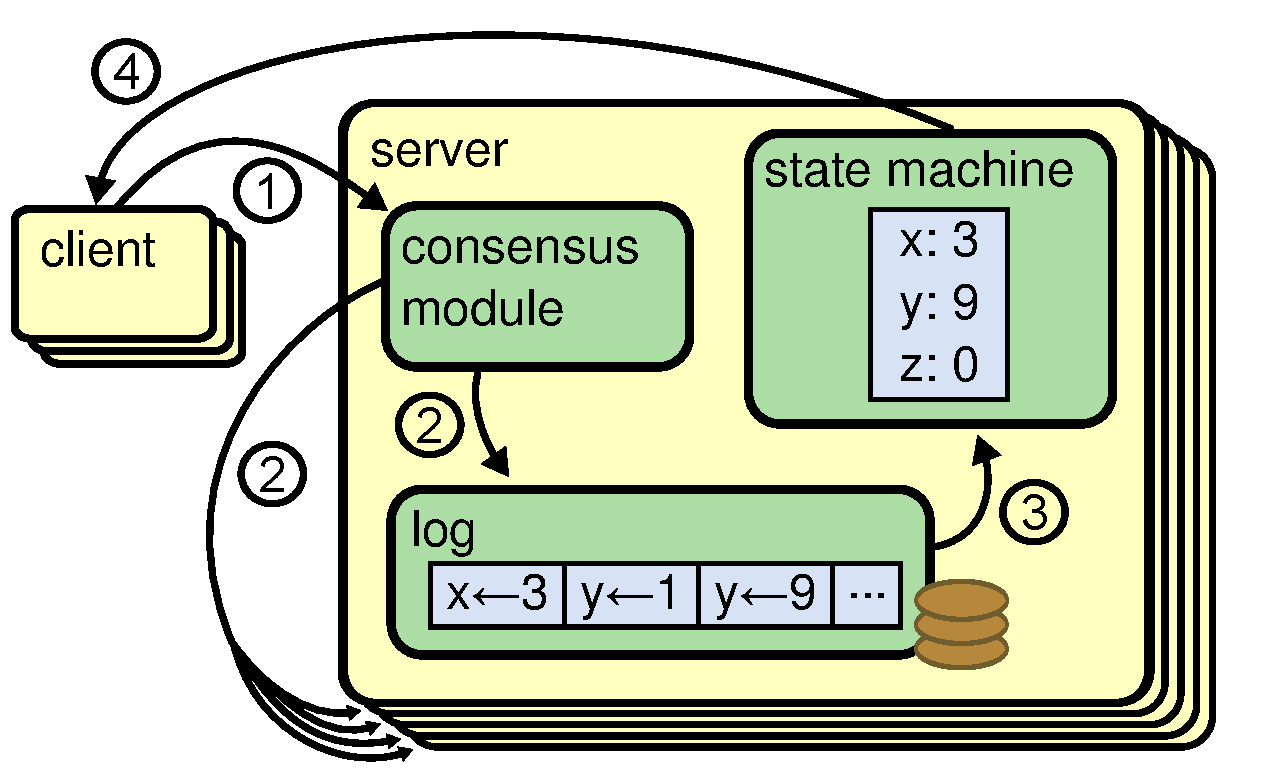
\includegraphics[width=0.80\columnwidth]{statemachine}
		\caption{Un modello di state machine semplificato}
		\label{fig:figure1}
	\end{figure}
